%\subsection{Purpose of this section}

This section gives advice on how to start your DP training processes using the framework. Moreover, it provides insights into how input pre-processing, building networks with Residual connections and Loss-logits gradient clipping could help offer better utility for the same privacy budget. 

\subsection{Prerequisite: building a $\ell$-Lipschitz network}

    As per def~\ref{def:feedforwardlipnet} a $l$-Lipschitz neural network of depth $d$ can be built by composing $\sqrt[\leftroot{3} \uproot{2} d]{l}$ layers. In the rest of this section we will focus on 1-Lipschitz networks (rather than controlling $l$ we control the loss to obtain the same effects \cite{bethune2022pay}). In order to do so the strategy consists in choosing only 1-Lipschitz activations, and to constrain the weights of parameterized layers such that it can only express 1-Lipschitz functions. For instance normalizing the weight matrix of a dense layer by its spectral norm yield a 1-Lipschitz layer (this, however cannot be applied trivially on convolution's kernel). In practice we used the layers available in the open-source library \textit{deel-lip}. In practice, when building a Lipschitz network, the following block can be used:
    
    \begin{itemize}
        \item Dense layers: are available as \textit{SpectralDense} or \textit{QuickSpectralDense} which apply spectral normalization and Bj\"orck orthogonalization, making them GNP layers.
        \item \textit{Relu} activations are replaced by \textit{Groupsort2} activations, and such activations are GNP, preventing vanishing gradient.
        \item pooling layers are replaced with \textit{ScaledL2NormPooling}, which is GNP since it performs the operation $x\mapsto (\|x_m\|_2)_m$ where $m$ is the multi-index of a patch of contiguous pixels.
        \item normalization layers like \textit{BatchNorm} are not $K$-Lipschitz. We did not accounted these layers since they can induce a privacy leak (as they keep a rolling mean and variance). A 1-Lipschitz drop-in replacement is studied in~\ref{ap:layernorm}. The relevant literature also propose drop-in replacement for this layer with proper sensitivity accounting.
    \end{itemize}

    Originally, this library relied on differentiable re-parametrizations, since it yields higher accuracy outside DP training regime (clean training without noise). However, our framework does not account for the Lipschitz constant of the re-parametrization operator. This is why we provide \textit{QuickSpectralDense} and \textit{QuickSpectralConv2D} layers to enforce Lipschitz constraints, where the projection is enforced with a tensorflow constraint. Note that \textit{SpectralDense} and \textit{SpectralConv2D} can still be used with a \textit{CondenseCallack} to enforce the projection, and bypass the back-propagation through the differentiable re-parametrization. However this last solution, while being closer to the original spirit of deel-lip, is also less efficient in speed benchmarks.  

    The Lipschitz constant of each layer is bounded by $1$, since each weight matrix is divided by the largest singular value $\sigma_{\text{max}}$. This singular value is computed with Power Iteration algorithm. Power Iteration computes the largest singular value by repeatedly computing a Rayleigh quotient asssociated to a vector $u$, and this vector eventually converges to the eigenvector $u_{\max}$ associated to the largest eigenvalue. These iterations can be expensive. However, since gradient steps are smalls, the weight matrices $W_t$ and $W_{t+1}$ remain close to each other after a gradient step. Hence their largest eigenvectors tend to be similar. Therefore, the eigenvector $u_{\max}$ can be memorized at the end of each train step, and re-used as high quality initialization at the next train step, in a ``lazy'' fashion. This speed-up makes the overall projection algorithm very efficient.   

\subsection{Getting started}

The framework we propose is built to allow DP training of neural networks in a fast and controlled approach. The tools we provide are the following :

\begin{enumerate}
    \item \textbf{A pipeline} to efficiently load and pre-process the data of commonly used datasets like MNIST, FashionMNIST and CIFAR10. 
    \item \textbf{Configuration objects} to correctly account DP events we provide config objects to fill in that will 
    \item \textbf{Model objects} on the principle of Keras' model classes we offer both a \lstinline[basicstyle=\ttfamily, backgroundcolor=\color{gray!20}]{DP_Model} and a \lstinline[basicstyle=\ttfamily, backgroundcolor=\color{gray!20}]{DP_Sequential} class to streamline the training process. 
    \item \textbf{Layer objects} where we offer a readily available form of the principal layers used for DNNs. These layers are already Lipschitz constrained and possess class specific methods to access their Lipschitz constant. 
    \item \textbf{Loss functions}, identically, we offer DP loss functions that automatically compute their Lipschitz constant for correct DP enforcing.
\end{enumerate}

We highlight below an example of a full training loop on Mnist with \textbf{lip-dp} library. Refer to the ``examples'' folder in the library for more detailed explanations in a jupyter notebook.  

\begin{center}
\begin{lstlisting}[language=Python,
basicstyle=\ttfamily\footnotesize,
stringstyle=\color{red}\ttfamily,
commentstyle=\color{olive}\ttfamily,
showstringspaces=false,
breaklines=true,
frame=lines,
classoffset=1,
morekeywords={compile, fit},
keywordstyle=\color{purple}\bfseries,
classoffset=2,
morekeywords={DP_Sequential, DP_BoundedInput, DP_QuickSpectralConv2D,
DP_GroupSort, DP_ScaledL2NormPooling2D,
DP_LayerCentering, DP_Flatten, DP_QuickSpectralDense,
DP_ClipGradient, MulticlassHinge, Adam, DP_Accountant, DPParameters},
keywordstyle=\color{blue}\bfseries,
classoffset=3,
morekeywords={input_shape, upper_bound, filters, kernel_size, strides, pool_size, loss, optimizer, epochs, batch_size, validation_data, callbacks, kernel_initializer, use_bias, drop_remainder, bound_fct, delta, noise_multiplier, noisify_strategy, metrics, dp_parameters, dataset_metadata},
keywordstyle=\color{gray}\bfseries,]
dp_parameters = DPParameters(
    noisify_strategy="global",
    noise_multiplier=2.0,
    delta=1e-5,
)

epsilon_max = 3.0

input_upper_bound = 20.0
ds_train, ds_test, dataset_metadata = load_and_prepare_data(
    "mnist",
    batch_size=1000,
    drop_remainder=True,
    bound_fct=bound_clip_value(
        input_upper_bound
    ),
)

# construct DP_Sequential
model = DP_Sequential(
    layers=[
        layers.DP_BoundedInput(
            input_shape=dataset_metadata.input_shape, upper_bound=input_upper_bound
        ),
        layers.DP_QuickSpectralConv2D(
            filters=32,
            kernel_size=3,
            kernel_initializer="orthogonal",
            strides=1,
            use_bias=False,
        ),
        layers.DP_GroupSort(2),
        layers.DP_ScaledL2NormPooling2D(pool_size=2, strides=2),
        layers.DP_QuickSpectralConv2D(
            filters=64,
            kernel_size=3,
            kernel_initializer="orthogonal",
            strides=1,
            use_bias=False,
        ),
        layers.DP_GroupSort(2),
        layers.DP_ScaledL2NormPooling2D(pool_size=2, strides=2),
        
        layers.DP_Flatten(),
        
        layers.DP_QuickSpectralDense(512),
        layers.DP_GroupSort(2),
        layers.DP_QuickSpectralDense(dataset_metadata.nb_classes),
    ],
    dp_parameters=dp_parameters,
    dataset_metadata=dataset_metadata,
)

model.compile(
    loss=losses.DP_TauCategoricalCrossentropy(18.0),
    optimizer=tf.keras.optimizers.SGD(learning_rate=2e-4, momentum=0.9),
    metrics=["accuracy"],
)
model.summary()

num_epochs = get_max_epochs(epsilon_max, model)

hist = model.fit(
    ds_train,
    epochs=num_epochs,
    validation_data=ds_test,
    callbacks=[
        # accounting is done thanks to a callback
        DP_Accountant(log_fn="logging"),
    ],
)
\end{lstlisting}
\end{center}

\subsection{Image spaces and input clipping}

Input preprocessing can be done in a completely dataset agnostic way (i.e without privacy leakages) and may yield positive results on the models utility. We explore here the choice of the color space, and the norm clipping of the input.

\subsubsection{Color space representations}

The color space of images can yield very different gradient norms during the training process. Therefore, we can take advantage of this to train our DP models more efficiently. Empirically, Figures~\ref{fig:histcolorspaceinput} and~\ref{fig:histcolorspacegrad} show that some color spaces yield narrower image norm distributions that happen to be more advantageous to maximise the mean gradient norm to noise ratio across all samples during the DP training process of GNP networks.

\subsubsection{Input clipping} 

A clever way to narrow down the distribution of the dataset's norms would be to clip the norms of the input of the model. This may result in improved utility since a narrower distribution of input norms might maximise the mean gradient norm to noise ratio for misclassified examples. Also, we advocate for the use of GNP networks as their gradients usually turn out to be closer to the upper bound we are able to compute for the gradient. See Figure~\ref{fig:histgradsallnet} and~\ref{fig:histgradsgnp} 


    \label{app:input_processing}
    \begin{figure}
    \begin{subfigure}{.45\columnwidth}
        \centering
        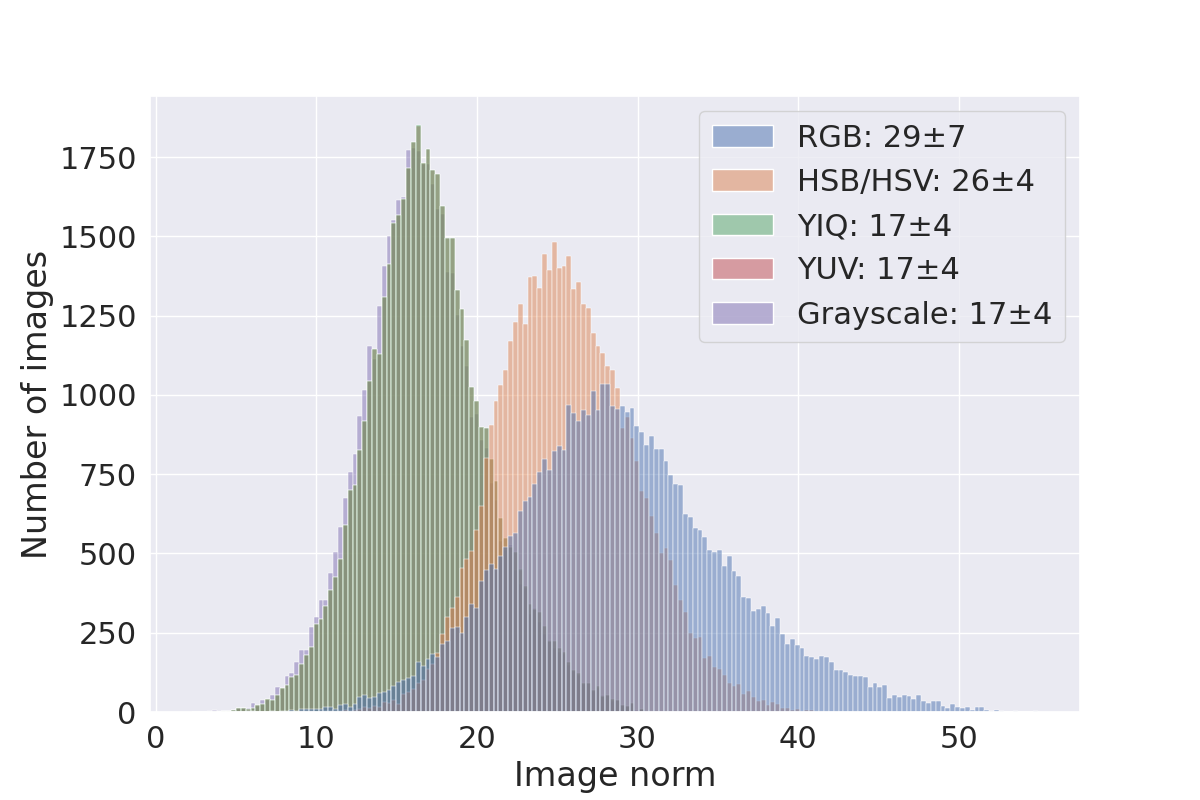
\includegraphics[width=\linewidth]{figures/Input_Space_Norms.PNG}
        \caption{Input norms.}
    \label{fig:histcolorspaceinput}
    \end{subfigure}
    \hfil
    \begin{subfigure}{.45\columnwidth}
        \centering
        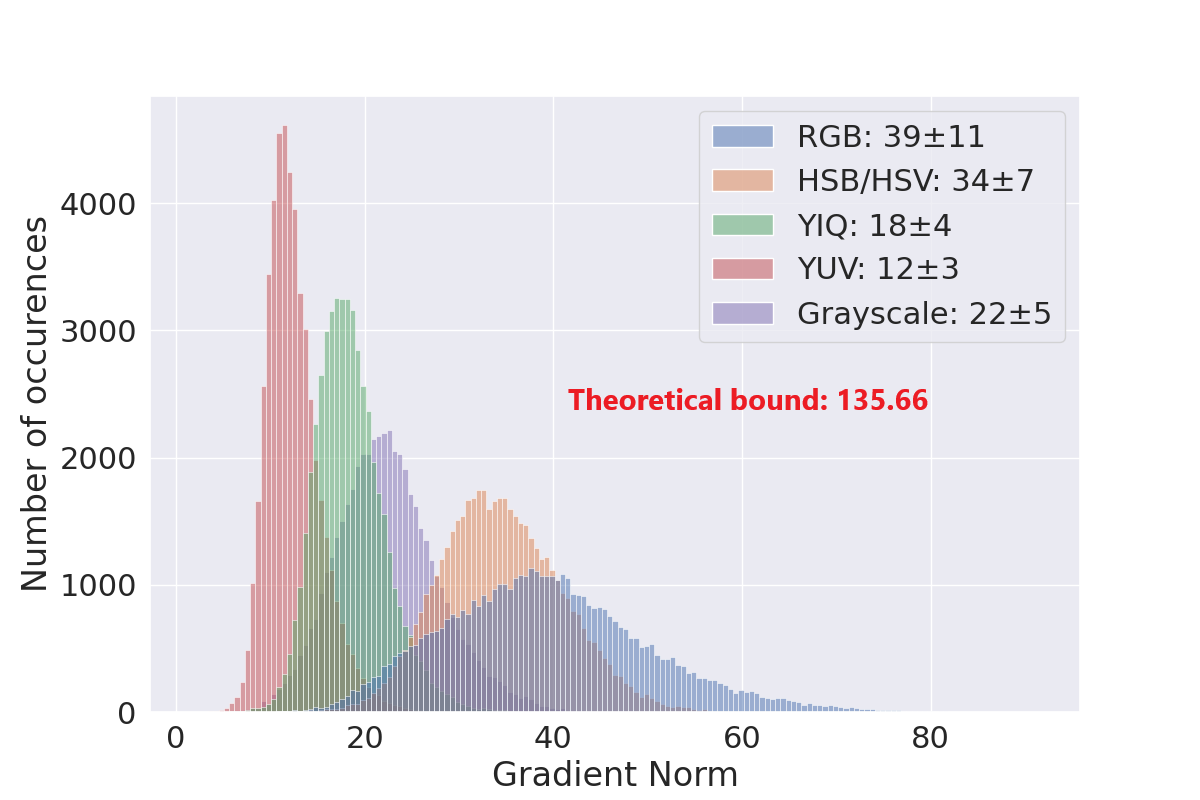
\includegraphics[width=\linewidth]{figures/Input_Space_Gradients.PNG}
        \caption{Gradient norms.}
    \label{fig:histcolorspacegrad}
    \end{subfigure}
    \caption{\textbf{Histogram of norms for different image space on CIFAR-10 images}. We see that for GNP networks the distribution of dataset norms have a strong influence on the norm of the individual parameterwise gradient norms of missclassified examples. The global gradient bound is equal to $135.66$ on this architecture: less than two times the maximum empirical bound of 73.}\label{fig:histcolorspace}
    \end{figure}

    \begin{figure}
    \begin{subfigure}{.45
\columnwidth}
    \centering
    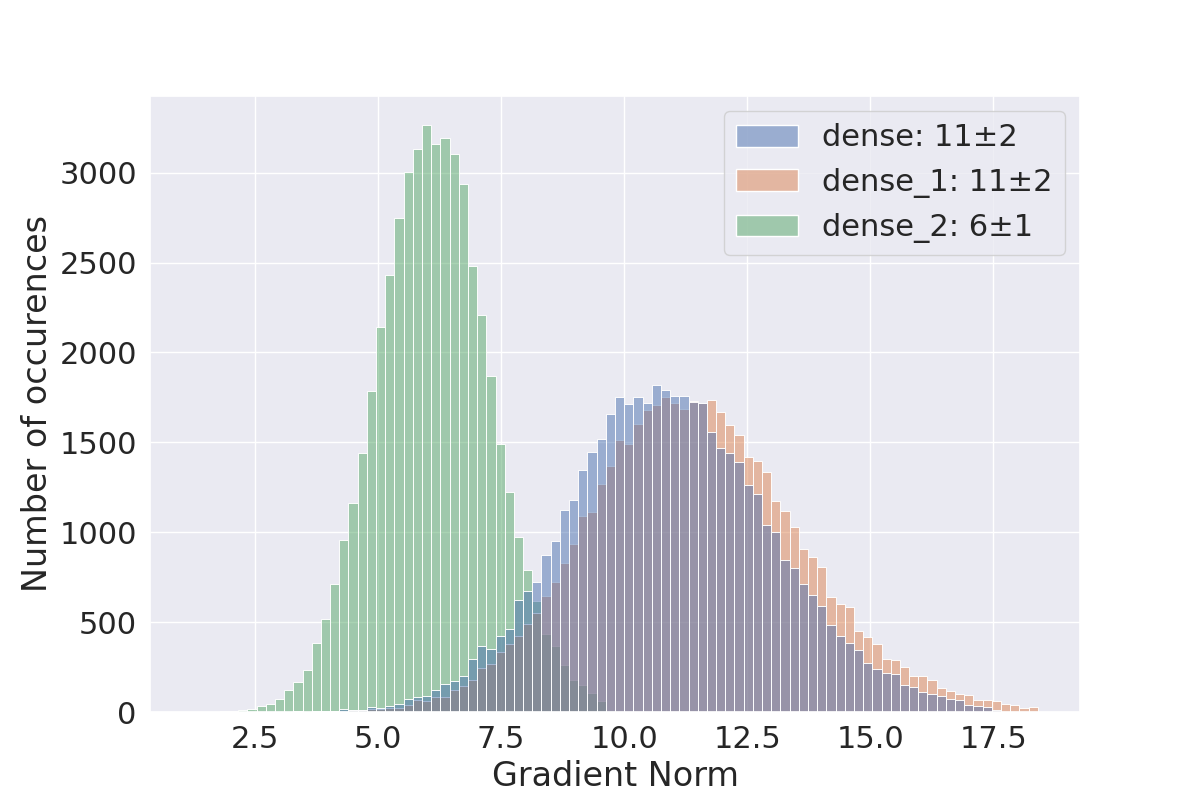
\includegraphics[width=\linewidth]{figures/Non-GNP_LayerGrads.PNG}
    \caption{Conventional network.}
    \label{fig:histgradsallnet}
\end{subfigure}
\hfil
\begin{subfigure}{.45\columnwidth}
    \centering
    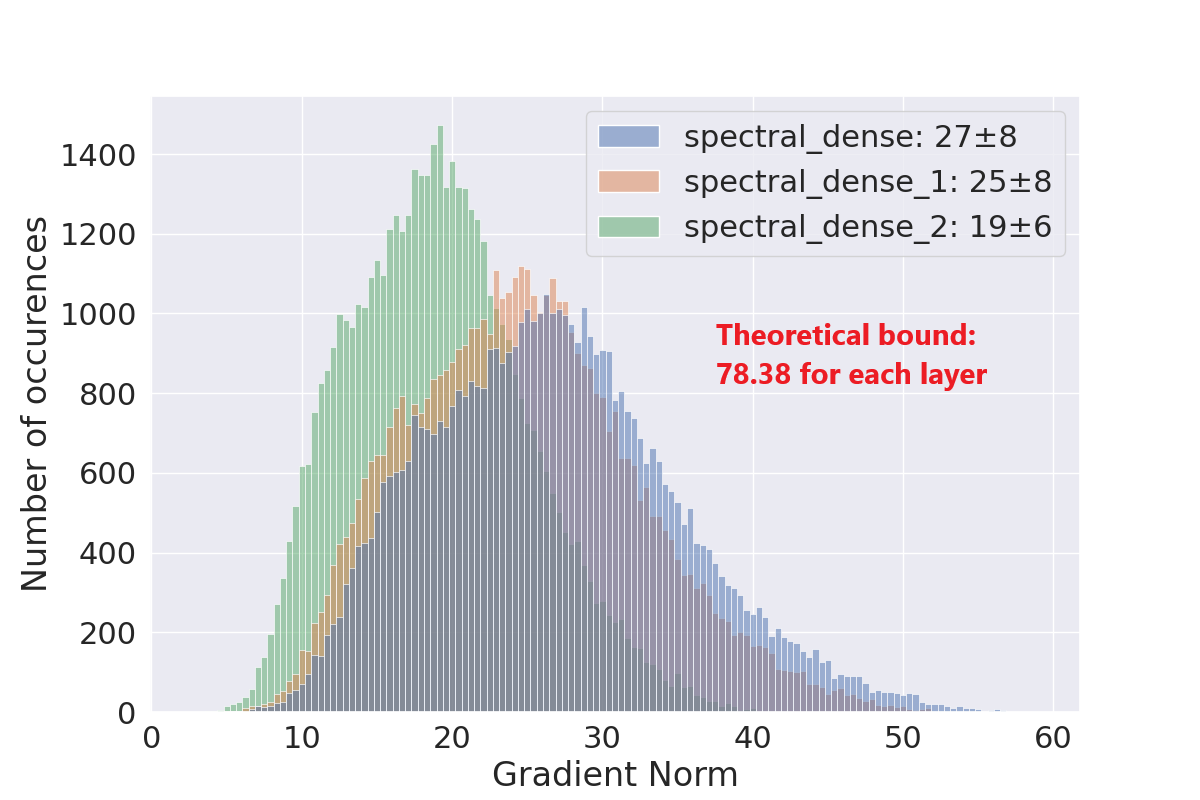
\includegraphics[width=\linewidth]{figures/GNP_LayerGrads.PNG}
    \caption{Gradient Norm Preserving network.}
    \label{fig:histgradsgnp}
\end{subfigure}
\caption{\textbf{Gradient norms of fully-connected networks on CIFAR-10}. We see that GNP networks exhibit a qualitatively different profile of gradient norms with respect to parameters, sticking closer to the upper bound we are able to compute for the gradient norm. The GNP network does not use biases, therefore all layers hare the same bound of $78.38$ for their gradient norm. Not too far away from the maximum empirical bound of 56 at initialization.}\label{fig:histgrad}
\end{figure}    

\subsection{Practical implementation of Residual connections}

The implementation of skip connections is made relatively straightforward in our framework by the \lstinline[basicstyle=\ttfamily, backgroundcolor=\color{gray!20}]{make_residuals} method. This function splits the input path in two, and wraps the layers inside the residual connections, as illustrated in figure~\ref{fig:residuals}.

\begin{center}
\begin{lstlisting}[language=Python,
basicstyle=\ttfamily\footnotesize,
stringstyle=\color{red}\ttfamily,
commentstyle=\color{olive}\ttfamily,
showstringspaces=false,
breaklines=true,
frame=lines,
classoffset=1,
morekeywords={compile, fit},
keywordstyle=\color{purple}\bfseries,
classoffset=2,
morekeywords={DP_Sequential, DP_BoundedInput, DP_QuickSpectralConv2D,
DP_GroupSort, DP_ScaledL2NormPooling2D,
DP_LayerCentering, DP_Flatten, DP_QuickSpectralDense,
DP_ClipGradient, MulticlassHinge, Adam, DP_Accountant, DPParameters, make_residuals},
keywordstyle=\color{blue}\bfseries,
classoffset=3,
morekeywords={input_shape, upper_bound, filters, kernel_size, strides, pool_size, loss, optimizer, epochs, batch_size, validation_data, callbacks, kernel_initializer, use_bias, drop_remainder, bound_fct, delta, noise_multiplier, noisify_strategy, metrics, dp_parameters, dataset_metadata},
keywordstyle=\color{gray}\bfseries,]
from lipdp.layers import make_residuals
## Manual implementation of residual connection:
layers = [DP_SplitResidual(),
          DP_WrappedResidual(DP_QuickSpectralConv2D(16, (3, 3)),
          DP_WrappedResidual(DP_GroupSort(2)),
          DP_MergeResidual('1-lip-add')]
## Or equivalently, with helper function:
layers = make_residuals([
    DP_QuickSpectralConv2D(16, (3, 3),
    DP_GroupSort(2)
 ])
\end{lstlisting}
\end{center}

\begin{figure}
        \centering
        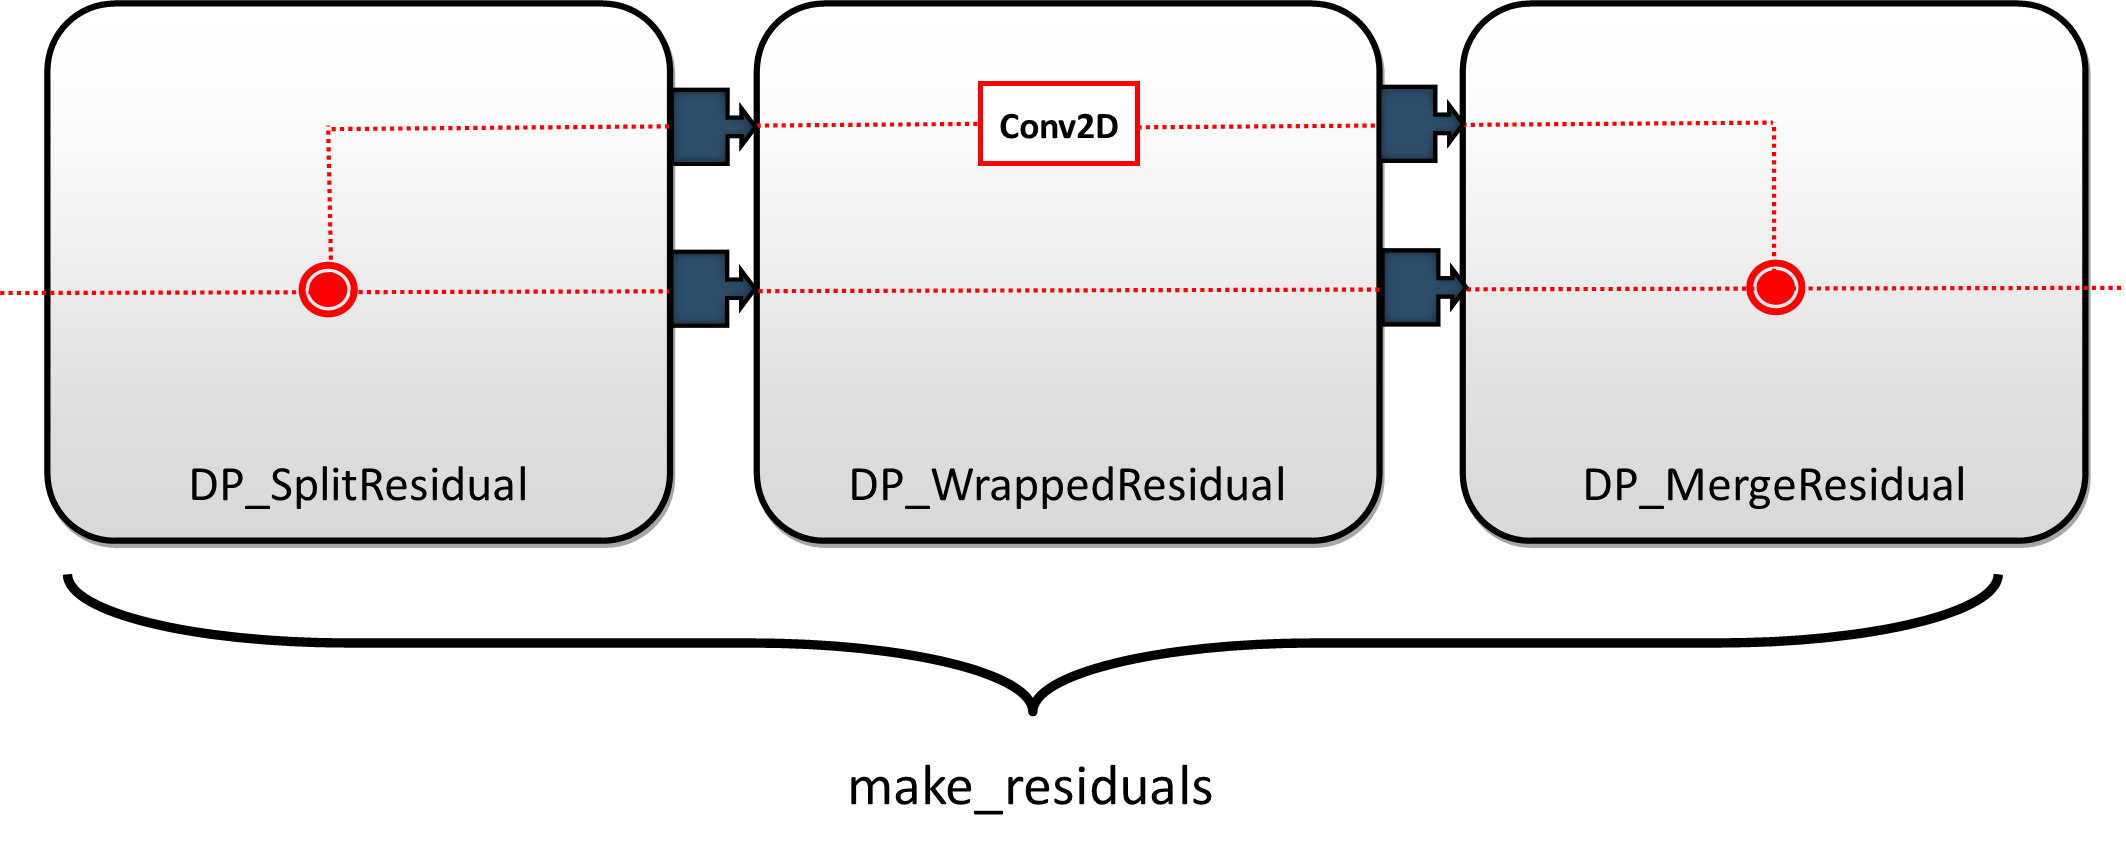
\includegraphics[width=\linewidth, height=5cm]{figures/residuals.png}
        \caption{Implementation of a skip connection in the \textbf{lip-dp} framework. The meta block \textbf{DP\_WrappedResidual} handle the forward propagation and the backward propagation of pairs of bounds (one for each computation path) by leveraging the forward and the backward of sub-blocks. \textbf{DP\_SplitResidual} handle the creation of a tuple of input bounds at the forward, and collapse the tuple of gradient bounds into a scalar at the backward, while \textbf{DP\_MergeResidual} does the opposite. All those operations are wrapped under the convenience function \textbf{make\_residuals}.}
        \label{fig:residuals}
\end{figure}

By using this implementation, the sensitivity of the gradient computation and the input bounds to each layer are correctly computed when the model's path is split. This allows for fairly easy implementations of models like the MLP-Mixer and ResNets. Since convolutional models may suffer from gradient vanishing and that dense based models are relatively restrictive in terms of architecture, implementing skip connections could be a useful feature for our framework.

% \begin{lstlisting}[language=Python,
% basicstyle=\ttfamily\small,
% stringstyle=\color{red}\ttfamily,
% commentstyle=\color{green}\ttfamily,
% showstringspaces=false,
% breaklines=true,
% frame=lines,
% classoffset=1,
% morekeywords={compile, fit},
% keywordstyle=\color{purple}\bfseries,
% classoffset=2,
% morekeywords={DP_Sequential, DP_BoundedInput, DP_SpectralConv2D,
% DP_GroupSort, DP_ScaledL2NormPooling2D,
% DP_LayerCentering, DP_Flatten, DP_SpectralDense,
% DP_ClipGradient, MulticlassHinge, Adam, DP_Accountant},
% keywordstyle=\color{blue}\bfseries,
% classoffset=3,
% morekeywords={input_shape, upper_bound, filters, kernel_size, pool_size, loss, optimizer, epochs, batch_size, validation_data, callbacks},
% keywordstyle=\color{gray}\bfseries,]
% model = DP_Sequential(
%     [
%         DP_BoundedInput(input_shape=(28, 28, 1), upper_bound=20.),
%         DP_SpectralConv2D(filters=16, kernel_size=3),
%         DP_GroupSort(2),
%         DP_ScaledL2NormPooling2D(pool_size=2, strides=2),
%         DP_LayerCentering(),
%         DP_Flatten(),
%         DP_SpectralDense(10),
%         DP_ClipGradient(0.1)
%     ],
%     noisify_strategy='local'
% )
% model.compile(loss=MulticlassHinge(0.05), optimizer=Adam(1e-3))
% model.fit(
%     x_train, y_train,
%     validation_data=(x_test, y_test),
%     epochs=num_epochs,
%     batch_size=512,
%     callbacks=[DP_Accountant()]
% )
% \end{lstlisting}

\subsection{Loss-logits gradient clipping}

    The advantage of the traditional DP-SGD approach is that through hyperparameter optimization on the global gradient clipping constant, we indirectly optimize the mean signal to noise ratio on missclassified examples. However, this clipping constant is not really explainable and rather just an empirical result of optimization on a given architecture and loss function. 

    Importantly, our framework is compatible with a more efficient and explainable form of clipping. As more and more examples are correctly classified, the magnitude of $\textcolor{backwardcolor}{\|\nabla_f \Loss\|}$ tend to diminish over the course of training, quickly falling below the upper bound and diminishing the gradient norm to noise standard deviation ratio. Gradient clipping strategy is still available in our framework. But instead of clipping the parameter gradient $\nabla_{\theta}\Loss$, any intermediate gradient $\nabla_{f_d}\Loss$ can be clipped during backpropagation. Indeed, by introducing a ``\textit{clipping layer}'' that behave like identity function at the forward pass, and clip the gradient during the backward pass, we are able to clip the gradient of the loss on the final logits for a minimal cost.  
    
    Indeed, in this case the size of the clipped vector is the output dimension $|\hat y|$, which is small for a lot of practical regression and classification tasks. For example in CIFAR-10 the output vector is of length $10$. This scales better with the batch size than the weight matrices that are typically of sizes~${64\times 64}$ or ${128\times 128}$. More precisely, in vanilla DP-SGD the per-weight gradient clipping is applied on the batched gradient $\nabla_{W_d}\Loss$ which is a tensor of size $b\times h^2$ for matrix weight~${W_d\in\Reals^{h\times h}}$. In privacy it is not unusual to have $b$ and $h$ in the $[10^2,10^4]$ range. Clipping this vector can cause memory issues or slowdowns~\cite{lee2021scaling}. However $\nabla_f\Loss$ is of size $b\times h$ which is significantly cheaper to clip. Note that the resulting ``gradient'' vector is not a true gradient anymore in a strictly mathematical sense, but rather a ``descent direction''~\cite{boyd2004convex}.  
    
    Furthermore, if the gradient clipping layer is inserted on the tail of the network (between the logits and the loss) we can characterize its effects on the training, in particular for classification tasks with binary cross-entropy loss.  

    We denote by $\Loss(\text{Clip}^C_{\nabla}(\hat y))$ the loss wrapped under a \textbf{DP\_ClipGradient} layer that behaves like identity $x\mapsto x$ at the forward, and clips the gradient norm to $C>0$ in the backward pass:
    \begin{align}
        \nabla_{\hat y}\left(\Loss(\text{Clip}^C_{\nabla}(\hat y))\right)\defeq& \min{(1,\frac{C}{\|\nabla_{\hat y}\Loss(\hat y)\|})}\nabla_{\hat y}\Loss(\hat y)\\ 
        =&\min{(\|\nabla_{\hat y}\Loss(\hat y)\|,C)}\frac{\nabla_{\hat y}\Loss(\hat y)}{\|\nabla_{\hat y}\Loss(\hat y)\|}.
    \end{align}
    We denote by $\overrightarrow{g(\hat y)}$ the unit norm vector $\frac{\nabla_{\hat y}\Loss(\hat y)}{\|\nabla_{\hat y}\Loss(\hat y)\|}$. Then:
    \[
        \nabla_{\hat y}\left(\Loss(\text{Clip}^C_{\nabla}(\hat y))\right) = \min{(\|\nabla_{\hat y}\Loss(\hat y)\|,C)}\overrightarrow{g(\hat y)}.
    \]

    \begin{restatable}[Clipped binary cross-entropy loss is the Wasserstein dual loss]{proposition}{bceiswass}\label{prop:bceiswass}
    Let $\Loss_{BCE}(\hat y,y)=-\log{(\sigma(\hat yy))}$ be the binary cross-entropy loss, with $\sigma(\hat yy)=\frac{1}{1+\exp{(-\hat yy)}}$ the sigmoid activation, assuming discrete labels~${y\in\{-1,+1\}}$. Assume examples are sampled from the dataset $\Dataset$. Let $\hat y(\theta, x)=f(\theta,x)$ be the predictions at input $x\in\Dataset$. Then for every $C>0$ sufficiently small, a gradient descent step with the clipped gradient $\nabla_{\theta}\Expect_{\Dataset}[\Loss(\text{Clip}^C_{\nabla}(\hat y,y))]$ is identical to the  
    gradient ascent step obtained from Kantorovich-Rubinstein loss $\Loss_{KR}(\hat y, y)=\hat yy$.  
    \end{restatable}
    \begin{proof}
    In the following we use the short notation $\Loss$ in place of $\Loss_{BCE}$. Assume that examples with labels $+1$ (resp. $-1$) are sampled from distribution $P$ (resp. $Q$).
    By definition:
    \begin{equation*}
         \nabla_{\theta}\Expect_{\Dataset}[\Loss(\text{Clip}^C_{\nabla}(\hat y,y))] = \nabla_{\theta}\left(\Expect_{x\sim P}[\Loss(\text{Clip}^C_{\nabla}(f(\theta, x),+1))]+\Expect_{x\sim Q}[\Loss(\text{Clip}^C_{\nabla}(f(\theta, x),-1))]\right).
    \end{equation*}
    Observe that the output of the network is a single scalar, hence $\overrightarrow{g(\hat y)}\in\{-1,+1\}$. We apply the chainrule $\nabla_{\theta}\Loss=\nabla_{\hat y}\Loss\Jac{\hat y}{\theta}=\overrightarrow{g(\hat y)}\min{(\|\nabla_{\hat y}\Loss(\hat y)\|,C)}\nabla_{\theta}f(\theta, x)$. We note $R(\hat y,C)\defeq\min{(\|\nabla_{\hat y}\Loss(\hat y)\|,C)}>0$ and we obtain:
    \begin{equation}
        \nabla_{\theta}\Expect_{\Dataset}[\Loss(\text{Clip}^C_{\nabla}(\hat y,y))] = \nabla_{\theta}\left(\Expect_{x\sim P}[\overrightarrow{g(\hat y)}R(\hat y,C)\nabla_{\theta}f(\theta, x)]+\Expect_{x\sim Q}[\overrightarrow{g(\hat y)}R(\hat y,C)\nabla_{\theta}f(\theta, x)]\right).
    \end{equation}
    Observe that the value of $\overrightarrow{g(\hat y)}$ can actually be deduced from the label $y$, which gives:
    \begin{equation}
        \nabla_{\theta}\Expect_{\Dataset}[\Loss(\hat y,y)] = -\Expect_{x\sim P}[R(\hat y,C)\nabla_{\theta}f(\theta, x)]+\Expect_{x\sim Q}[R(\hat y,C)\nabla_{\theta}f(\theta, x)].
    \end{equation}
    Observe that the function $x\mapsto \nabla_{\hat y}\Loss(\hat y)$ is piecewise-continuous when the loss $\hat y\mapsto \Loss(\hat y, y)$ is piecewise continuous. Observe that $|\nabla_{\hat y}\Loss(\hat y)|$ is non zero, since the loss $\Loss$ does not achieve its minimum over the open set $(-\infty,+\infty)$, since $\sigma(\hat y)\in (0,1)$. Assuming that the data $x\in\Dataset$ lives in a compact space (or equivalently that $P$ and $Q$ have compact support), since $x\mapsto|\nabla_{\hat y}\Loss(\hat y)|$ is piecewise continuous (with finite number of pieces for finite neural networks) it attains its minimum $C'>0$. Choosing any $C<C'$ implies that $R(\hat y, C)=C$, which yields:
    \begin{align*}
        \nabla_{\theta}\Expect_{\Dataset}[\Loss(\text{Clip}^C_{\nabla}(\hat y,y))] &= -\Expect_{x\sim P}[C\nabla_{\theta}f(\theta, x)]+\Expect_{x\sim Q}[C\nabla_{\theta}f(\theta, x)]\\
        &= -C\left(\Expect_{x\sim P}[\nabla_{\theta}f(\theta, x)]-\Expect_{x\sim Q}[\nabla_{\theta}f(\theta, x)]\right).
    \end{align*}
    This corresponds to a gradient \textit{ascent} step of length $C$ on the Kantorovich-Rubinstein (KR) objective $\Loss_{KR}(\hat y, y)=\hat yy$. This loss is named after the Kantorovich Rubinstein duality that arises in optimal transport, than states that the Wasserstein-1 distance is a supremum over 1-Lipschitz functions:
    \begin{equation}
        \mathcal{W}_1(P,Q)\defeq\underset{f\in\text{1-Lip}(\Dataset,\Reals)}{\sup}\Expect_{x\sim P}[f(x)]-\Expect_{x\sim Q}[f(x)].
    \end{equation}
    Hence, with clipping $C$ small enough the gradient steps are actually identical to the ones performed during the estimation of Wasserstein-1 distance.  
    \end{proof}
  
    The adaptive clipping of~\cite{andrew2021differentially} takes the form of a Gaussian mechanism so the implementation of the RDP accountant is straightforward. 

    In future works, other multi-class losses can be studied through the lens of per-example clipping. Our framework permits the use of gradient clipping while at the same time faciliting the theoretical anaysis.  

\subsubsection{Possible improvements}

Our framework is compatible with possible improvements in methods of data pre-processing. For instance some works suggest that feature engineering is the key to achieve correct utility/privacy trade-off \cite{tramer2021differentially} some other work rely on heavily over-parametrized networks, coupled with batch size \cite{de2022unlocking}. While we focused on providing competitive and reproducible baselines (involving minimal pre-processing and affordable compute budget) our work is fully compatible with those improvements.
Secondly the field of GNP networks (also called orthogonal networks) is still an active field, and new methods to build better GNP networks will improve the efficiency of our framework ( for instance orthogonal convolutions \cite{achour2022existence},\cite{li2019orthogonal},\cite{li2019preventing},\cite{trockman2021orthogonalizing},\cite{singla2021skew} are still an active topic).
Finally some optimizations specific to our framework can also be developed: a scheduling of loss-logits clipping might allow for better utility scores by following the declining value of the gradient of the loss, therefore allowing for a better mean signal to noise ratio across a diminishing number of miss-classified examples. Observe that our framework is also compatible with other ideas, such as the progressing freezing of deeper layers proposed by~\cite{tang2022dp}.  
